\section{Introduction}
\label{sec:intro}

Sports organisations now collect force-plate data as routinely as they collect attendance. A squad can be put through a set of countermovement jumps (CMJs) in a few minutes, the software returns jump height, peak force, impulses and phase durations within seconds, and those numbers flow into dashboards that coaches and physiotherapists use to plan training, judge readiness and decide when an injured player can return \parencite{claudino2017,gathercole2015,cormack2008}. The appeal is obvious. A handful of numbers can be tracked over a season, compared between players and set against targets.

What the dashboard does not show is the force--time curve from which those numbers were taken. Each jump produces thousands of force samples, and every summary metric is a single point, an area or a duration read off that curve. Two athletes can reach the same height with different patterns of force: one sinks quickly and pushes hard for a short time, the other descends slowly and pushes for longer. If such differences are common, a report built on jump height and peak force treats as equivalent athletes who are not, and a coach who wants to change how an athlete jumps receives no guidance on where in the movement to look \parencite{mcmahon2018,floria2019}. The same concern applies to the landing, which the plates record in every trial but which most monitoring reports reduce to one peak value or ignore.

This paper asks one question of routine CMJ records from male football players at a private performance centre in India: at which points along take-off and landing do jumps differ systematically, and what do the conventional metrics fail to capture? We treat each phase as a curve and use methods from functional data analysis that test every instant of the movement while controlling the error rate over the whole curve \parencite{ramsay2005,pataky2015}. The sample is dominated by adolescents, which brings a second, practical question: do differences between younger and older players reflect age itself, or simply the size and jump height that come with it?

The contribution is not a new statistical method. It is a careful reading of a dataset of the kind many organisations already hold, with the athlete rather than the trial treated as the unit of evidence, so that players who were tested often do not dominate the conclusions. We show where along the curve better jumpers differ, that jumps of the same height can be produced with different curves, that the apparent groups of `jump strategies' are better described as a continuum, and that the landing carries information no take-off metric supplies. Section~\ref{sec:lit} reviews the relevant work, Section~\ref{sec:methods} sets out data and methods, Section~\ref{sec:findings} reports the findings, and Section~\ref{sec:conclusion} draws out implications and limitations.

\section{Literature review}
\label{sec:lit}

Studies of the CMJ have long tried to find which discrete variables separate good and poor jumpers. The answer has been consistently disappointing. No single kinetic or temporal variable accounts for performance on its own \parencite{dowling1993}, and the variables that vendors report are correlated with one another and with body size \parencite{mcmahon2018,laffaye2014}. Their reliability also varies: jump height and peak force are repeatable between days, while rate-based and time-based variables are less so \parencite{hori2009}. For monitoring, the practical consequence is that a change in one metric can arise from several different changes in the way the athlete moved.

Waveform analysis was proposed as a way around the choice of variables. Analysing the whole time-normalised curve, through principal components or functional principal components, lets the data reveal which parts of the movement vary \parencite{ramsay2005,warmenhoven2019}. Applied to the CMJ, these methods have shown that better jumpers produce more force late in the propulsive phase and that the unweighting and braking phases contain information that discrete variables miss \parencite{richter2014,floria2019,parker2018}. In on-water rowing, \textcite{warmenhoven2018} compared functional principal components, statistical parametric mapping (SPM) and discrete analysis on the same force profiles and found that the conclusions depended on the method, with the curve-based approaches locating differences that discrete values could only summarise. Reviews of functional methods in biomechanics now treat function-on-scalar regression and SPM as complementary tools \parencite{gunning2024,morris2015}: the first estimates how a scalar such as jump height relates to force at each instant, the second tests group differences at each instant with control of the family-wise error rate \parencite{pataky2012,pataky2015,nichols2002}.

Three methodological issues recur in this literature and shape the present design. The first is time. CMJ phases differ in duration between and within athletes, so curves must be brought to a common time base before they can be compared. Linear normalisation to a fixed number of nodes is the usual choice, but it mixes differences in timing with differences in force; landmark registration and elastic alignment separate the two, and their use changes the strength and location of jump-height effects \parencite{moudy2018,white2022,pataky2022,white2020isbs}. Registration is not neutral either, because the warping itself may carry performance information. The second issue is dependence. Monitoring data contain several trials per session and several sessions per athlete, and treating trials as independent inflates the evidence. Functional mixed models with athlete-level random curves \parencite{di2009,goldsmith2011,scheipl2015,morris2006} and resampling of athletes rather than trials address this, but few CMJ studies have used them. The third is grouping. Clustering curves is an appealing way to sort athletes into `strategies' \parencite{jacques2014}, and the principal component structure of CMJ curves can itself shift over a season \parencite{kipp2015isbs}. Yet clustering algorithms return groups whether or not any exist, so evidence for discrete strategies depends on validation that is often missing \parencite{hennig2007,tibshirani2001}.

The landing has received far less attention. It is recorded in every trial and loads the lower limb more heavily than take-off, yet even injury-related waveform work has looked at take-off: in elite athletes tested before and after anterior cruciate ligament reconstruction, SPM found force deficits at the end of propulsion that discrete values missed \parencite{acl2025}. Whether landing curves differ with performance or with age in young players has not, to our knowledge, been examined with whole-curve methods. Youth samples bring a further difficulty: age, body mass and jump height rise together during adolescence, and strength qualities develop unevenly with maturation \parencite{lloyd2012,malina2015}, so an apparent age effect on the curve may reflect size or performance rather than age itself.

This study therefore draws on the waveform literature but applies it to a routine monitoring dataset, with athlete-level inference throughout, two independent estimation approaches for every curve-wide claim, explicit checks of the time-normalisation choices, and validation before any clustering result is interpreted.

\section{Methodology}
\label{sec:methods}

\subsection{Data, setting and quality control}

The data are CMJ trials recorded during routine assessment of male football players at a private sports physiotherapy and performance centre in India between \testPeriod, shared with the authors under a non-disclosure and data-sharing agreement. All such trials in the centre's account were exported, giving \nTrialsAll{} trials from \nAthAll{} athletes in \nSessAll{} sessions, where a session is one visit at which an athlete jumped once or more. Identifiers were replaced by pseudonymous codes before analysis, and age at test was derived before dates were removed. \ethics{The study was approved by [Ethics committee name, approval number and date to be inserted]. [Written informed consent was obtained from adult athletes, and written consent from a parent or guardian, together with the athlete's assent, was obtained for athletes under 18 years.] / [The committee waived the requirement for consent for the secondary use of de-identified routine monitoring data.] [Delete the option that does not apply.] The study conformed to the Declaration of Helsinki.}

Jumps were performed on dual force plates (VALD ForceDecks, VALD Performance, Brisbane, Australia) sampling at 1000\,Hz (\nFsHigh{} analysed trials) or 500\,Hz (\nFsLow). Testing followed the centre's routine, so warm-up, instructions and rest intervals were not recorded and no landing technique was prescribed. The software supplied jump height from flight time, concentric peak force, eccentric braking impulse, the concentric impulse over the first 100\,ms, peak landing force, contraction time and flight time; these are the conventional metrics against which the curves are compared. Five quality-control rules removed trials with a missing or invalid body mass (R1), a quiet-stance mass more than 5\% away from the recorded mass (R2), mean force above 50\,N during flight (R3), a missing metric or age (R4), or no identifiable lowest centre-of-mass position after touch-down (R5). The rules removed \nDropped{} trials and \nAthLost{} athletes, leaving \nTrials{} trials from \nAth{} athletes in \nSess{} sessions (Table~\ref{tab:desc}). Ages ranged from \ageMin{} to \ageMax{} years (median \ageMedian), \pctUnderEighteen\% of trials came from players under 18, and \nAthMulti{} athletes were tested in two or more sessions.

% Generated by explore_fda/make_paper_outputs.R -- regenerate rather than edit
\begin{table}[!htbp]
\centering
\begin{threeparttable}
\caption{Sample characteristics}
\label{tab:desc}
\footnotesize\setlength{\tabcolsep}{3pt}
\begin{tabular}{@{}l S[table-format=4.2] S[table-format=3.2] S[table-format=4.2] S[table-format=4.2] S[table-format=4.2] S[table-format=4.2] S[table-format=4.2]@{}}
\toprule
 & & & & \multicolumn{2}{c}{Quartiles} & \multicolumn{2}{c}{Range} \\
\cmidrule(lr){5-6}\cmidrule(l){7-8}
Variable & {Mean} & {SD} & {Median} & {Q1} & {Q3} & {Min} & {Max} \\
\midrule
\multicolumn{8}{@{}l}{\textit{Athletes ($n$ = 212)}} \\
\quad Age at first test (years) & 16.0 & 5.9 & 14.1 & 12.0 & 16.8 & 8.8 & 37.9 \\
\quad Body mass at first test (kg) & 53.3 & 15.9 & 51.7 & 40.9 & 64.0 & 25.0 & 96.0 \\
\quad Trials per athlete & 3.8 & 2.3 & 3.0 & 2.0 & 5.0 & 1.0 & 16.0 \\
\quad Sessions per athlete & 1.5 & 0.8 & 1.0 & 1.0 & 2.0 & 1.0 & 6.0 \\
\addlinespace
\multicolumn{8}{@{}l}{\textit{Sessions ($n$ = 327)}} \\
\quad Trials per session & 2.5 & 0.8 & 2.0 & 2.0 & 3.0 & 1.0 & 7.0 \\
\addlinespace
\multicolumn{8}{@{}l}{\textit{Trials ($n$ = 805)}} \\
\quad Jump height (cm) & 28.2 & 8.4 & 27.0 & 21.6 & 34.7 & 8.5 & 51.5 \\
\quad Concentric peak force (BW) & 2.35 & 0.38 & 2.29 & 2.11 & 2.51 & 1.65 & 4.70 \\
\quad Eccentric braking impulse (N\,s) & 27.8 & 15.4 & 24.6 & 16.6 & 35.7 & 0.0 & 95.2 \\
\quad Concentric impulse, first 100\,ms (N\,s) & 62.2 & 26.7 & 58.7 & 41.8 & 79.1 & 1.5 & 187.9 \\
\quad Peak landing force (BW) & 5.39 & 1.97 & 4.97 & 3.88 & 6.67 & 2.19 & 14.88 \\
\quad Take-off duration (s) & 0.78 & 0.19 & 0.77 & 0.66 & 0.90 & 0.31 & 1.48 \\
\quad Landing duration (s)$^{a}$ & 0.25 & 0.11 & 0.24 & 0.15 & 0.31 & 0.07 & 0.93 \\
\quad Native samples, take-off$^{b}$ & 755 & 212 & 762 & 627 & 889 & 180 & 1484 \\
\quad Native samples, landing$^{b}$ & 238 & 116 & 223 & 144 & 310 & 41 & 928 \\
\bottomrule
\end{tabular}
\begin{tablenotes}[flushleft]\footnotesize
\item \textit{Note.} BW = multiples of body weight. Take-off runs from movement onset to take-off (vendor contraction time). 59 trials were recorded at 500\,Hz and 746 at 1000\,Hz. $^{a}$Touch-down to the lowest point of the centre of mass. $^{b}$Phase duration multiplied by the sampling rate; each phase is resampled to 101 nodes.
\end{tablenotes}
\end{threeparttable}
\end{table}


\subsection{From force records to comparable curves}

The take-off phase runs from movement onset $t_{\mathrm{on}}$ to take-off $t_{\mathrm{to}} = t_{\mathrm{on}} + T_{\mathrm{c}}$, where $T_{\mathrm{c}}$ is contraction time. The landing phase runs from touch-down $t_{\mathrm{td}} = t_{\mathrm{to}} + T_{\mathrm{f}}$, with $T_{\mathrm{f}}$ the flight time, to the lowest point of the centre of mass, the first instant after touch-down at which vertical velocity, obtained by integrating net force from an initial value of $-g T_{\mathrm{f}}/2$, returns to zero \parencite{linthorne2001,street2001,mcmahon2018}. Force was divided by body weight and each phase was linearly resampled to 101 equally spaced nodes,
\begin{equation}
y_{ij}(s) = \frac{F_{ij}\{t_{0,ij} + s\,(t_{1,ij} - t_{0,ij})\}}{m_i\,g}, \qquad s \in \{0, 0.01, \ldots, 1\},
\label{eq:norm}
\end{equation}
where $F_{ij}$ is the summed vertical force in trial $j$ of athlete $i$, $m_i$ the body mass recorded with the trial, $g = 9.81$\,m\,s$^{-2}$, and $[t_{0,ij}, t_{1,ij}]$ the phase limits. Results are expressed in multiples of body weight (BW) at a given percentage of the phase \parencite{richter2014,warmenhoven2019}.

The node count was chosen from the data rather than by convention. Take-off phases contained between \toSampMin{} and several thousand native samples (median \toSampMedian), so 101 nodes downsample every take-off. Landings were much shorter (median \ldSampMedian{} samples), and \nLdUnder{} landings (\pctLdUnder\%) had fewer than 101, so for them the grid interpolates rather than samples. Resampling at 101 nodes kept a median of \retLdMedian{} of the native peak landing force, whereas a 51-node grid would have lost up to \decLossLdP\% of the peak in the worst 1\% of landings. Three checks showed that the choice did not drive the results. Re-interpolating the stored curves to 51 and 201 nodes, with linear or spline interpolation, and repeating the main analyses moved the boundaries of significant regions by one or two percentage points, left the landing group comparison \nodeSpmLdSame, and changed cumulative component variance by at most \nodePcMaxDiff{} percentage points; linear and spline values at grid midpoints differed by a median of \splineDiffMedian{}\,BW. A velocity check confirmed the event definitions: take-off velocity integrated from the force record correlated $r = \velR$ with the value implied by flight time.

Linear normalisation treats a difference in timing as a difference in force. We examined this in two ways. Landmark registration added minimum and zero centre-of-mass velocity as interior landmarks in take-off, and peak landing force in landing, warping each curve piecewise-linearly so that landmarks coincide \parencite{moudy2018,white2022}. Elastic alignment of landing curves used the square-root velocity framework \parencite{srivastava2011,tucker2013}, in which each curve $f$ is represented by $q(s) = \operatorname{sign}\{\dot f(s)\}\sqrt{|\dot f(s)|}$ and aligned to a Karcher mean by a warping function $\gamma$ that minimises $\lVert q_{\mu} - (q \circ \gamma)\sqrt{\dot\gamma} \rVert$. This splits variation into amplitude (aligned curves) and phase (the warps), which can then be analysed separately \parencite{pataky2022}.

\subsection{Where along the curve does force relate to performance?}

The main model is a function-on-scalar regression,
\begin{equation}
y_{ij}(s) = \beta_0(s) + \beta_{\mathrm{JH}}(s)\,z^{\mathrm{JH}}_{ij} + \beta_{\mathrm{age}}(s)\,z^{\mathrm{age}}_{ij} + \beta_{\mathrm{BM}}(s)\,z^{\mathrm{BM}}_{ij} + b_i(s) + c_{ij}(s) + \varepsilon_{ij}(s),
\label{eq:fosr}
\end{equation}
where the $z$ are jump height, age and body mass standardised to one SD (\sdJH\,cm, \sdAge{} years and \sdBM\,kg), $b_i(s)$ and $c_{ij}(s)$ are athlete and session random curves, and $\varepsilon_{ij}(s)$ is residual error. Each coefficient function $\beta_p(s)$ is the change in force, in BW, at instant $s$ for a one-SD difference in the predictor with the others held fixed. Body mass is in the model because heavier players jump differently in absolute terms and are, in this sample, older.

Equation~\eqref{eq:fosr} was estimated in two ways, and a region is reported only when both agree. The first fits ordinary least squares at each node and builds simultaneous 95\% bands from 2000 bootstrap resamples of athletes, so that all trials and sessions of an athlete are resampled together \parencite{efron1993}. The band is $\hat\beta_p(s) \pm \hat q\,\widehat{\mathrm{se}}(s)$, where $\hat q$ is the 95th percentile over resamples of $\max_s |\hat\beta^{*}_p(s) - \hat\beta_p(s)| / \widehat{\mathrm{se}}(s)$; it covers the whole function with 95\% probability rather than each node separately \parencite{ruppert2003}. The critical values ranged from \simCritMin{} to \simCritMax. The second approach fits the functional mixed model directly with penalised splines and athlete and session random curves \parencite{scheipl2015,goldsmith2011}, on every second node to keep the computation feasible, with simultaneous bands from the posterior covariance. The two approaches fail differently. The bootstrap is honest about dependence between trials but ignores smoothness; the mixed model uses smoothness, but its residuals were strongly autocorrelated along the curve (lag-one correlation \residLagMin--\residLagMax), so its bands are too narrow and it tends to find more regions. Requiring agreement guards against both.

To separate athletes who jump higher from jumps that are higher, jump height was also split into its athlete mean and the trial's deviation from it,
\begin{equation}
\mathrm{JH}_{ij} = \overline{\mathrm{JH}}_{i} + (\mathrm{JH}_{ij} - \overline{\mathrm{JH}}_{i}),
\label{eq:wb}
\end{equation}
and both parts entered the bootstrap model in place of jump height. The between-athlete term describes how better jumpers differ from poorer ones; the within-athlete term describes how the same athlete's curve changes on a better day.

\subsection{Group comparisons, profiles and their validation}

Group differences were tested with a permutation version of SPM applied to one mean curve per athlete, so that each athlete contributes once. At each node a Welch $t$ statistic compared the groups; adjacent nodes whose $|t|$ exceeded the two-sided 5\% threshold formed clusters, and each cluster's mass $\sum_{s \in c} |t(s)|$ was compared with the permutation distribution of the largest cluster mass over the whole phase,
\begin{equation}
p_c = \frac{1 + \#\{\,k : \max_{c'} M^{(k)}_{c'} \ge M_c\,\}}{1 + K}, \qquad K = 5000,
\label{eq:perm}
\end{equation}
which controls the family-wise error rate over all 101 nodes \parencite{nichols2002,maris2007,pataky2015}. Two contrasts were examined: athletes in the top versus the bottom tertile of mean jump height (\nTop{} versus \nBottom), and athletes aged 18 or over versus under 18 (\nAdult{} versus \nJunior). Because size and performance are confounded with group, each contrast was repeated after adjusting for the other two variables (age and body mass for the tertile contrast; body mass and jump height for the age contrast) by Freedman--Lane permutation of residuals \parencite{winkler2014}. Effect sizes are the mean difference at the node of largest $|t|$ and Hedges' $g$, both with 95\% intervals from 2000 bootstrap resamples of athletes within groups. With four primary tests, a Bonferroni threshold of \bonf{} is also reported.

A matched-height comparison asked the question managers most often ask of these data: if two players jump equally high, do they jump in the same way? Trials whose jump height lay between the 45th and 55th percentiles were compared with the whole sample on the spread of their curves and on the mix of curve profiles defined next.

Profiles were obtained by $k$-means clustering on functional principal component scores covering at least 90\% of variance, separately for take-off and landing \parencite{jacques2014}. Because $k$-means always returns groups, the clustering was treated as exploratory and validated with the mean silhouette width \parencite{kaufman1990}, the gap statistic with $k = 1$ allowed \parencite{tibshirani2001}, a dip test of unimodality of the leading score, and bootstrap cluster-wise Jaccard similarity \parencite{hennig2007}. The stability of profiles within athletes was measured as the share of athletes with two or more sessions whose profile was the same in every session, and compared with the share expected if profiles were assigned at random in proportion to their frequency, obtained by permuting labels within the sample. Profiles were not used to define the groups in the SPM tests, which avoids testing a difference created by the clustering itself. All analyses used R \parencite{rcore2026} with a fixed random seed.

\section{Findings}
\label{sec:findings}

\subsection{Where better jumpers differ}

Force rose to a first peak late in take-off and to a larger, more variable impact peak early in landing (Fig.~\ref{fig:fosr}A). Jump height was associated with force in two parts of take-off on which both estimation approaches agreed: early, at \supJHtoEarly\% of the phase, where higher jumpers unweighted more deeply (a negative coefficient), and late, from \supJHtoLateLo\% to \supJHtoLateHi\%, where they pushed harder (Table~\ref{tab:fosr}; Fig.~\ref{fig:fosr}B). The mixed model's band touched zero in \supJHtoGaps{} short stretches of the late window, which we do not claim. The largest effect was \pkJHto\,BW per SD of jump height at \pkJHtoat\% of take-off (95\% CI [\pkJHtolo, \pkJHtohi]). Age added almost nothing once jump height and body mass were in the model; its supported region was confined to about \supAgeTo\% of take-off, a coefficient of \pkAgeTo\,BW per SD.

\begin{figure}[!htbp]
\centering
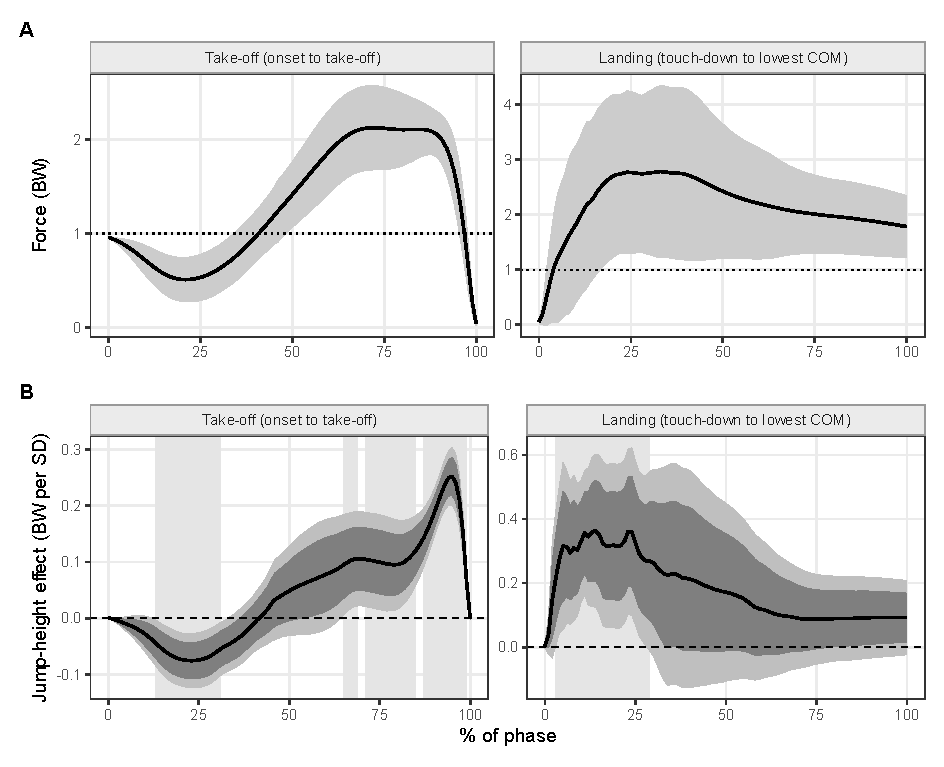
\includegraphics[width=\linewidth]{Fig1_mean_curves_fosr}
\caption{\capFosr}
\label{fig:fosr}
\end{figure}

% Generated by explore_fda/make_paper_outputs.R -- regenerate rather than edit
\begin{table}[!htbp]
\centering
\begin{threeparttable}
\caption{Regions of each phase where force was associated with jump height, age and body mass}
\label{tab:fosr}
\footnotesize
\begin{tabular*}{\linewidth}{@{\extracolsep{\fill}}>{\raggedright\arraybackslash}p{4.3cm} >{\raggedright\arraybackslash}p{4.1cm} S[table-format=2.0] S[table-format=-1.3] l@{}}
\toprule
Predictor & {Region (\% of phase)$^{a}$} & {Peak (\%)} & {Effect} & {95\% CI} \\
\midrule
\multicolumn{5}{@{}l}{\textit{Panel A. Take-off, effect in BW per SD of the predictor}} \\
\quad Jump height & {14--30, 66--68, 72--84, 88--98} & 95 & 0.25 & {[0.22, 0.29]} \\
\quad Age & {98} & 98 & 0.09 & {[0.06, 0.12]} \\
\quad Body mass & {2--6, 98--100} & 98 & -0.06 & {[$-$0.09, $-$0.03]} \\
\addlinespace
\multicolumn{5}{@{}l}{\textit{Panel B. Landing, effect in BW per SD of the predictor}} \\
\quad Jump height & {4--28} & 14 & 0.36 & {[0.21, 0.52]} \\
\quad Age & {--} & {--} & {--} & {--} \\
\quad Body mass & {76--82} & 78 & -0.18 & {[$-$0.30, $-$0.06]} \\
\addlinespace
\multicolumn{5}{@{}l}{\textit{Panel C. Jump height split within and between athletes, effect in BW per cm$^{b}$}} \\
\quad Take-off, between athletes & {18--29, 67--99} & 95 & 0.031 & {[0.026, 0.035]} \\
\quad Take-off, within athlete & {3--29, 46--63, 92--99} & 58 & 0.029 & {[0.017, 0.042]} \\
\quad Landing, between athletes & {9--15, 18--25} & 24 & 0.039 & {[0.016, 0.061]} \\
\quad Landing, within athlete & {2--16, 23} & 13 & 0.115 & {[0.074, 0.164]} \\
\bottomrule
\end{tabular*}
\begin{tablenotes}[flushleft]\footnotesize
\item \textit{Note.} Function-on-scalar regression of body-weight-normalised force on jump height, age and body mass, each standardised (1 \textit{SD} = 8.4\,cm, 5.7 years and 15.8\,kg). Effect is the coefficient at the peak of the region, with a pointwise 95\% confidence interval (CI) from 2000 bootstrap resamples of athletes. BW = multiples of body weight; dash = no region.
\item $^{a}$Panels A and B: nodes where the simultaneous 95\% bands of both the athlete-bootstrap least-squares fit and the functional mixed model (athlete and session random curves) exclude zero. $^{b}$Athlete-mean jump height and the trial's deviation from it entered together; region from the athlete-bootstrap simultaneous band.
\end{tablenotes}
\end{threeparttable}
\end{table}


In landing, higher jumps were followed by larger forces early in the phase, at \supJHld\% (largest effect \pkJHld\,BW per SD at \pkJHldat\%; 95\% CI [\pkJHldlo, \pkJHldhi]), and age had no supported effect anywhere. The model explained little of the landing curve: the pointwise $R^2$ lay between \rtwoLdMinA\% and \rtwoLdMaxA\%. Take-off was different. At \rtwoToShareLow\% of nodes between 5\% and 89\% of the phase, jump height, age and body mass together explained less than 10\% of the variance, but in the last tenth of take-off they explained up to \rtwoToLate\%. The conventional metrics are therefore informative about the end of the push and say little about the rest of the movement.

The split of jump height in Equation~\eqref{eq:wb} showed that the early-landing effect is largely a within-athlete matter. When an athlete jumped higher than his own average, early landing force rose by \wiLdCm\,BW per cm (95\% CI [\wiLdCmLo, \wiLdCmHi]; significant mainly at \wiLdFirst\% of the phase), about \wiBwRatio{} times the between-athlete effect of \bwLdCm\,BW per cm. Within-athlete variation in jump height was small (SD \sdJHwithin\,cm against \sdJHbetween\,cm between athlete means), but each extra centimetre on a given day came with a markedly harder landing. In take-off, within- and between-athlete effects were of similar size per centimetre (Table~\ref{tab:fosr}).

The group comparison of athlete-mean curves confirmed the late-push window (Table~\ref{tab:spm}; Fig.~\ref{fig:spm}). Athletes in the top jump-height tertile produced more force than those in the bottom tertile from \tertToReg\% of take-off ($p$ \tertToP). At \tertToAt\% the means were \tertToMeanHi{} and \tertToMeanLo\,BW, a difference of \tertToD\,BW (95\% CI [\tertToDlo, \tertToDhi]) and Hedges' $g$ of \tertToG{} [\tertToGlo, \tertToGhi]. After adjustment for age and body mass the difference remained, at \tertToAdjRegs. In landing the top tertile showed higher force over \tertLdReg\% of the phase ($p$ \tertLdP; difference \tertLdD\,BW [\tertLdDlo, \tertLdDhi] at \tertLdAt\%, $g$ = \tertLdG{} [\tertLdGlo, \tertLdGhi]), but after adjustment only \tertLdAdjReg\% remained, at $p$ = \tertLdAdjP, which does not pass the Bonferroni threshold. The landing difference between good and poor jumpers is thus weaker and partly explained by size.

\begin{figure}[!htbp]
\centering
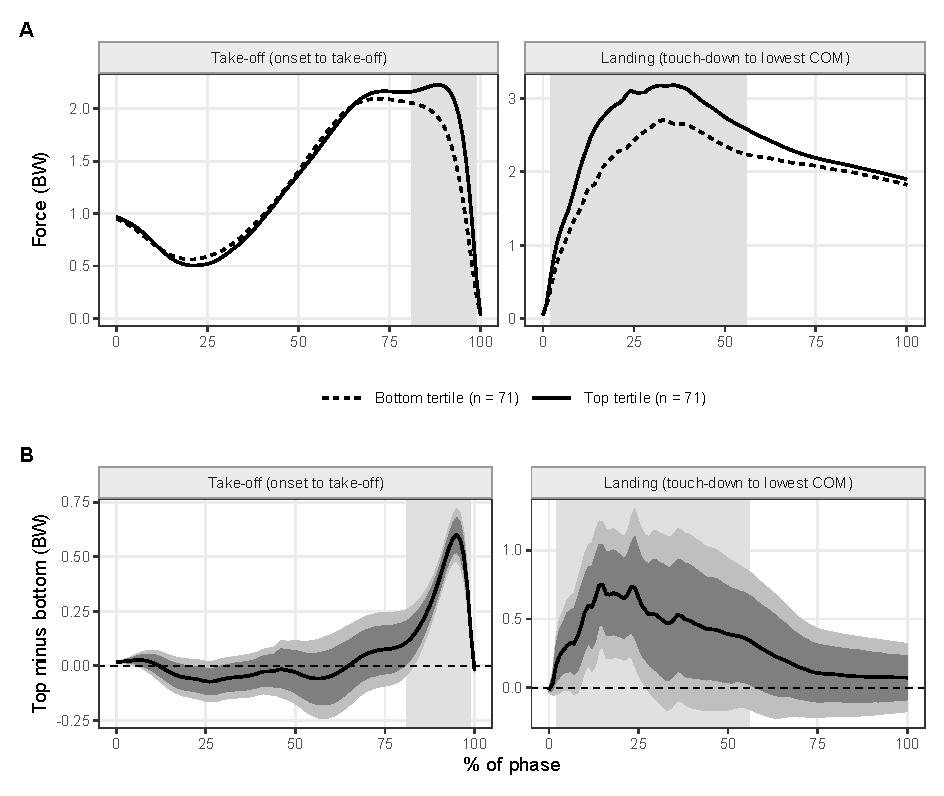
\includegraphics[width=\linewidth]{Fig2_tertile_comparison}
\caption{\capSpm}
\label{fig:spm}
\end{figure}

% Generated by explore_fda/make_paper_outputs.R -- regenerate rather than edit
\begin{table}[!htbp]
\centering
\begin{threeparttable}
\caption{Group differences in athlete-mean force curves}
\label{tab:spm}
\footnotesize
\begin{tabular*}{\linewidth}{@{\extracolsep{\fill}}l l c S[table-format=2.0] S[table-format=1.2] l S[table-format=1.2] l@{}}
\toprule
 & & & & \multicolumn{2}{c}{Difference (BW)} & \multicolumn{2}{c}{Hedges' \textit{g}} \\
\cmidrule(lr){5-6}\cmidrule(l){7-8}
Phase & {Region (\%)} & {\textit{p}} & {Peak (\%)} & {Value} & {95\% CI} & {Value} & {95\% CI} \\
\midrule
\multicolumn{8}{@{}l}{\textit{Panel A. Top vs bottom tertile of jump height (71 vs 71 athletes)}} \\
\quad Take-off & {81--99} & {$<$.001} & 93 & 0.55 & {[0.48, 0.61]} & 2.63 & {[2.31, 2.94]} \\
\quad Landing & {2--56} & .003 & 15 & 0.75 & {[0.45, 1.04]} & 0.83 & {[0.50, 1.15]} \\
\multicolumn{8}{@{}l}{\hspace{0.5em}\textit{Adjusted for age and body mass}$^{a}$} \\
\quad Take-off & {12--32} & .021 & {--} & {--} & {--} & {--} & {--} \\
\quad  & {66--99} & {$<$.001} & {--} & {--} & {--} & {--} & {--} \\
\quad Landing & {19--40} & .043 & {--} & {--} & {--} & {--} & {--} \\
\addlinespace
\multicolumn{8}{@{}l}{\textit{Panel B. Aged 18 or over vs under 18 (48 vs 164 athletes)}} \\
\quad Take-off & {87--99} & {$<$.001} & 96 & 0.47 & {[0.36, 0.56]} & 1.60 & {[1.25, 1.92]} \\
\quad Landing & {none} & .069$^{c}$ & {--} & {--} & {--} & {--} & {--} \\
\multicolumn{8}{@{}l}{\hspace{0.5em}\textit{Adjusted for body mass and jump height}$^{a}$} \\
\quad Take-off & {none} & .123$^{c}$ & {--} & {--} & {--} & {--} & {--} \\
\quad Landing & {none} & .226$^{c}$ & {--} & {--} & {--} & {--} & {--} \\
\bottomrule
\end{tabular*}
\begin{tablenotes}[flushleft]\footnotesize
\item \textit{Note.} One mean curve per athlete. Region = cluster of adjacent nodes (\% of the phase) where the groups differed; \textit{p} from 5000 permutations of the largest cluster mass, controlling the family-wise error rate over the phase$^{b}$. Peak = node of the largest |\textit{t}| in the region, where the difference (first group minus second; BW = multiples of body weight) and Hedges' \textit{g} are given with 95\% confidence intervals (CIs) from 2000 bootstrap resamples of athletes within groups. Bonferroni threshold for the four primary tests: \textit{p} < .0125.
\item $^{a}$Freedman--Lane permutation of residuals. $^{b}$Nodes with $|t|$ above the two-sided 5\% threshold form clusters. $^{c}$No significant region; smallest cluster \textit{p} shown.
\end{tablenotes}
\end{threeparttable}
\end{table}


\subsection{Age is mostly size and performance}

Adult players produced more force than under-18 players at the very end of take-off (\ageToReg\%, $p$ \ageToP; difference \ageToD\,BW [\ageToDlo, \ageToDhi], $g$ = \ageToG{} [\ageToGlo, \ageToGhi]), and showed no landing difference that survived family-wise control (the largest cluster, at \ageLdRawReg\%, had $p$ = \ageLdRawP). Once body mass and jump height were adjusted for, the take-off difference disappeared (smallest $p$ = \ageToAdjMinP). Older players push harder at the end of take-off because they are heavier and jump higher, not because of age as such.

\subsection{Same height, different curves}

The \bandN{} trials from \bandAth{} athletes with jump height between \bandLo{} and \bandHi\,cm were almost as varied in shape as the full sample: the pointwise SD of their curves was \bandSdRatioMin--\bandSdRatioMax{} times that of all trials (Fig.~\ref{fig:band}). Fixing jump height therefore removed almost none of the variation in how force was produced. Both take-off profiles and both landing profiles were present in the band in roughly their overall proportions (Table~\ref{tab:profiles}). Two players with the same jump height on a report may thus have produced it with a short, forceful take-off or a long, slower one, and absorbed the landing over a short or a long phase.

\begin{figure}[!htbp]
\centering
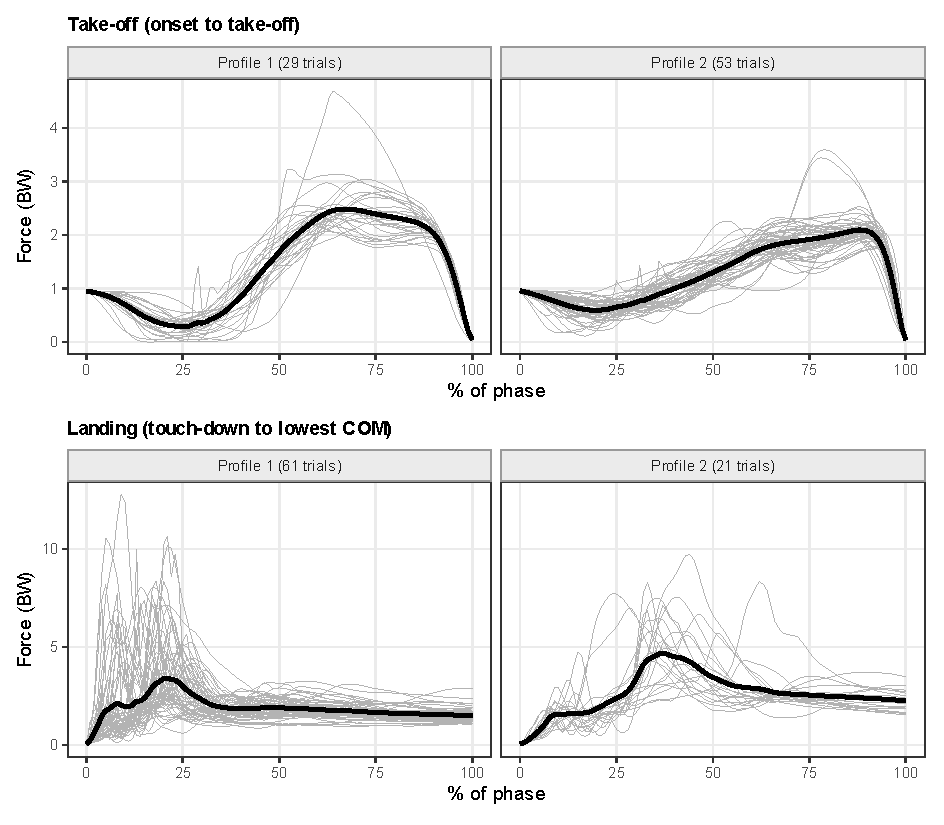
\includegraphics[width=\linewidth]{Fig3_matched_height}
\caption{\capBand}
\label{fig:band}
\end{figure}

\subsection{Profiles form a continuum, but landing habits persist}

The two-profile solution separated take-offs mainly by duration (mean \ctProfOneTo{} versus \ctProfTwoTo\,s) and landings by how quickly the impact was absorbed (mean landing duration \ldProfOneLd{} versus \ldProfTwoLd\,s). The validation did not support discrete strategies (Table~\ref{tab:profiles}; Fig.~\ref{fig:profiles}). Silhouette widths were low (\silTo{} and \silLd), the gap statistic preferred a single group for take-off and gave no clear answer for landing (\gapKLd{} groups, the largest number allowed), and the dip test found no departure from unimodality in either phase ($p$ = \dipTo{} and \dipLd). The profiles were reproducible in the sense that bootstrap resamples recovered them (mean Jaccard similarity \jacMinAll--\jacMaxAll), but a reproducible cut of a continuum is still a cut. We therefore read the profiles as the two ends of a continuous spectrum.

\begin{figure}[!htbp]
\centering
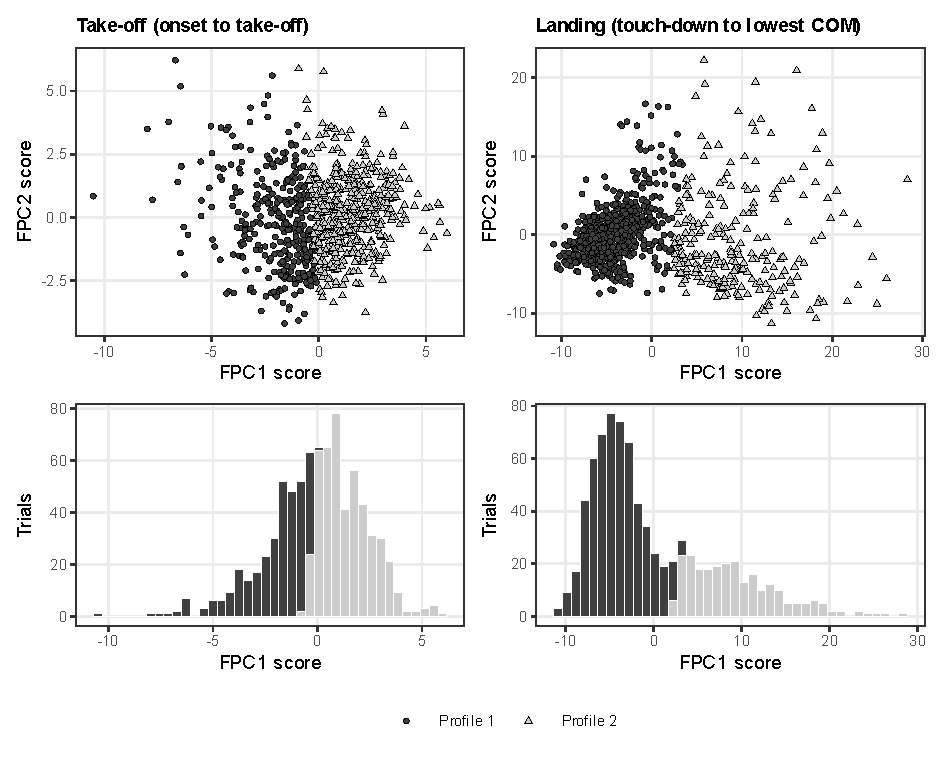
\includegraphics[width=\linewidth]{Fig4_profile_continuum}
\caption{\capProfiles}
\label{fig:profiles}
\end{figure}

% Generated by explore_fda/make_paper_outputs.R -- regenerate rather than edit
\begin{table}[!htbp]
\centering
\begin{threeparttable}
\caption{Curve profiles: description, validation and stability within athletes}
\label{tab:profiles}
\footnotesize\setlength{\tabcolsep}{4pt}
\begin{tabularx}{\linewidth}{@{}>{\raggedright\arraybackslash}X ll@{}}
\toprule
 & Take-off & Landing \\
\midrule
\multicolumn{3}{@{}l}{\textit{Description}} \\
\quad Profile 1 / profile 2 (trials) & 329 / 476 & 560 / 245 \\
\quad Mean jump height (cm) & 29.6 / 27.2 ($p$ < 0.001)$^{a}$ & 28.4 / 27.7 ($p$ = 0.017)$^{a}$ \\
\quad Mean take-off duration (s) & 0.65 / 0.87 & 0.79 / 0.76 \\
\quad Mean landing duration (s) & 0.24 / 0.25 & 0.29 / 0.14 \\
\addlinespace
\multicolumn{3}{@{}l}{\textit{Is there cluster structure?}} \\
\quad Mean silhouette & 0.30 & 0.37 \\
\quad Number of groups preferred by the gap statistic$^{b}$ & 1 & 6 \\
\quad Dip test of unimodality, first FPC score ($p$) & 0.74 & 0.98 \\
\quad Bootstrap Jaccard similarity (range over profiles) & 0.93--0.95 & 0.97--0.99 \\
\addlinespace
\multicolumn{3}{@{}l}{\textit{Stability}} \\
\quad Same profile in every session, \% (athletes with $\geq$ 2 sessions, $n$ = 83) & 55 & 70 \\
\quad Expected by chance, \% (permutation $p$) & 43 (0.007) & 51 ($<$0.001) \\
\quad Two trials in one session share a profile, \% (chance) & 76 (52) & 80 (58) \\
\quad Profile mix in the matched-height band, \% (all trials)$^{c}$ & 35 / 65 (41 / 59) & 74 / 26 (70 / 30) \\
\quad Agreement with profiles after elastic alignment (ARI) & {--} & 0.17 \\
\bottomrule
\end{tabularx}
\begin{tablenotes}[flushleft]\footnotesize
\item \textit{Note.} Profiles from $k$-means ($k$ = 2) on functional principal component (FPC) scores covering at least 90\% of variance, computed separately for each phase. $^{a}$Linear mixed model with an athlete random intercept. $^{b}$Candidates 1 to 6; 1 means no cluster structure. $^{c}$Trials with jump height between the 45th and 55th percentiles (26.0--28.2\,cm, 82 trials).
\end{tablenotes}
\end{threeparttable}
\end{table}


Where an athlete sat on that spectrum was nonetheless partly a stable trait, more so in landing than in take-off. Among the \nAthMulti{} athletes tested more than once, \stabLd\% kept the same landing profile in every session against \chanceLd\% expected by chance ($p$ \pStabLd); for take-off the figures were \stabTo\% and \chanceTo\% ($p$ \pStabTo). Elastic alignment showed why landing profiles should not be over-interpreted. Phase accounted for about \srvfPhaseShare\% of landing variance, the spread of peak timing fell from \srvfPeakSDun\% to \srvfPeakSDal\% of the phase after alignment, and profiles re-derived from aligned curves agreed only weakly with the original ones (adjusted Rand index \srvfAri). Much of what separates the landing profiles is therefore timing. The tertile difference in landing survived alignment (\srvfSpmA\%, $p$ = \srvfSpmAP), while the phase functions showed no group difference. Landmark registration gave the same picture: higher jumpers reached peak landing force earlier (\tmPeak\% of the phase per SD; 95\% CI [\tmPeaklo, \tmPeakhi]), and the landing tertile difference remained at \lmSpmLd\% ($p$ = \lmSpmLdP).

\section{Conclusion and implications}
\label{sec:conclusion}

The question was where along take-off and landing jumps differ, and what conventional metrics miss. The answer from these routine records is fairly clear. Better jumpers differ most in the late push, from about two-thirds of take-off to the moment of leaving the ground, with a smaller difference early in the unweighting; these regions were found by two estimation approaches, survived adjustment for age and body mass and were large in standardised terms. Outside the last tenth of take-off, jump height, age and body mass explained very little of the curve, and jumps of the same height came in shapes as varied as the whole sample. Landing differences were smaller, partly explained by size and largely a matter of timing, but the way an athlete lands was a more stable habit than the way he takes off. Apparent age differences reflected size and performance.

These findings agree with waveform studies that place performance differences in the propulsive phase \parencite{richter2014,floria2019,warmenhoven2018}, and they add evidence from a youth-dominated monitoring sample analysed at the athlete level. They temper the language of distinct `jump strategies': with validation, the profiles in our data looked like regions of a continuum, a result that warns against reading cluster labels as athlete types \parencite{hennig2007}. The within-athlete landing effect, which is about \wiBwRatio{} times the between-athlete effect per centimetre, suggests that on days when an athlete jumps higher he also lands harder, a pattern that day-to-day monitoring could follow.

\subsection*{Implications for practice and management}

For managers of high-performance programmes, the first implication concerns training emphasis. If force in the final third of take-off is what separates better jumpers, programmes that aim to raise jump height should target the ability to keep producing force as the legs extend, and progress should be judged by changes in that window rather than in jump height alone. The second concerns reporting. A single number hides how it was achieved, so the curve, or at least a late-push and an early-landing summary taken from it, should sit beside jump height in athlete reports. The cost is negligible, because the plates already record the full curve. Third, in youth programmes landing load rises with jump height within the same athlete; coaches who push a young player for height should watch how that player lands, and the persistence of landing profiles across sessions suggests that landing habits can be identified and tracked. Whether a short, stiff landing raises injury risk is a hypothesis that these data cannot test, and it should not be used for selection decisions. Fourth, benchmarks for young players should be adjusted for body size and performance; comparing a 14-year-old with an adult on unadjusted curve features will mostly measure growth \parencite{lloyd2012,malina2015}. More broadly, the analysis shows what a performance organisation can learn by reading data it already owns at a finer grain, without new equipment or testing.

\subsection*{Limitations}

Several limitations follow from the use of routine data. Testing was not standardised for research, filtering applied by the vendor software is unknown, and low-pass filtering is known to alter CMJ metrics \parencite{harry2022}. Short landings were interpolated rather than sampled: \pctLdUnder\% had fewer than 101 native samples, and resampling cut the native peak landing force by more than 2\% in \retLdPctTwo\% of trials. Quality control was not neutral, as the dropped trials came from lighter athletes (mean \bmDropped{} versus \bmKept\,kg, $p$ = \pBmDropped) with lower jumps (\jhDropped{} versus \jhKept\,cm, $p$ = \pJhDropped), so the smallest players are slightly under-represented. Trials per athlete were uneven, with the most-tested tenth of athletes contributing \pctTopTen\% of trials; athlete-level resampling and athlete-mean comparisons limit their influence, and trial- and athlete-weighted estimates of the jump-height effect correlated at \wcorJHto{} in take-off and \wcorJHld{} in landing. The sample is male, mostly adolescent and from one centre, maturation status was not recorded, and the design is cross-sectional, so causal and injury-related claims are beyond its reach. Future work should link curve features to training interventions and injury records over time.
